Consider now the case in which, as in step 3, the conversion rates are unknown but also the values of the graph weights.\\ This parameters gave us the probability with which a customer clicks on the secondary product, after he has as primary product another product.\\ Therefore, we initialize both the leraners (UCB-1 and TS) with the graph weights all set to 1.\\ 
In the same way as the previous step, here below we reported the addictional calculus to estimate the new unknown parameters, since from step 1 to 5 for UCB-1 and from step 1 to 4 for TS, they are both the same as in the third scenario.

\subsection{UCB-1}
As said before the first five step are the same, so here is reported how the graph weights are estimated:
\begin{equation}
    estimated\_graph[p,:] = \frac{estimated\_graph[p,:] * bought[p] + clicks[p,:]}{tot\_bought[p]}
\end{equation}where \begin{itemize}
    \item estimated\_graph[p,:] we are considering all the weights of the graph that starts from the node with the product {\bf p}
    \item bought[p] is the number of times the product {\bf p} has been bought until the day before
    \item clicks[p,:] is the row of the matrix that reports the number of times an edge of the graph has been activated, that means that a click on the secondary product (columns) has been recorded given a primary product (row). So here we look at all the edge that has been activated starting by the primary profuct {\bf p}
    \item tot\_bought[p] is the number of times the product {\bf p} has been bought until today (so it is bought[p] plus the number of times product p has been bought today)
\end{itemize}
\subsection{TS}
In this case the Thomson Sampling does exactly the same as the UCB-1 to estimate the graph weights.
\subsection{Results}
Also about the results we can say that are at most the same as the provious step: both algorithms performs a little bit worst compared to the case in which only one parameters were uncertain (conversion rates).\\ Another think that remains unchanged is that TS performed better than UCB-1 by reaching the optimal super arm faster.
\begin{figure}[ht]
    \begin{center}
    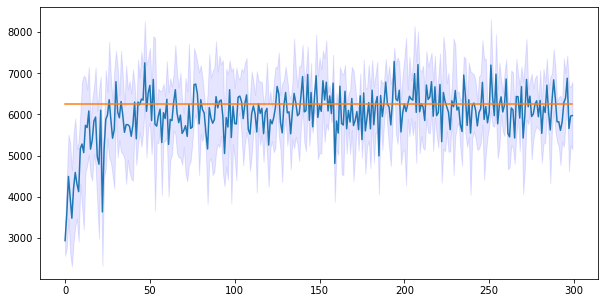
\includegraphics[width=0.6\textwidth]{img/ucb_reward5.png}
    \caption{UCB Reward}
    \label{fig:reward51}
    \end{center}
\end{figure}
\begin{multicols}{2}
    \begin{figure}[H]
        \begin{center}
        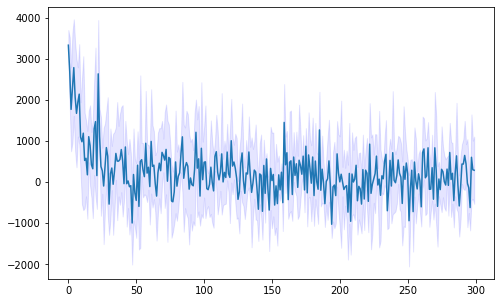
\includegraphics[width=0.5\textwidth]{img/ucb_regret5.png}
        \caption{UCB Regret}
        \label{fig:regret51}
        \end{center}
    \end{figure}
    \columnbreak
    \begin{figure}[H]
        \begin{center}
        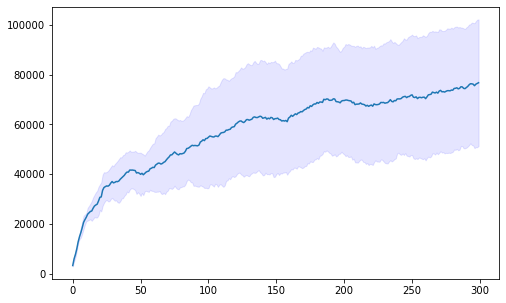
\includegraphics[width=0.5\textwidth]{img/ucb_cum_regret5.png}
        \caption{UCB Cumulative regret}
        \label{fig:cum_reg51}
        \end{center}
    \end{figure}
\end{multicols}
\begin{figure}[ht]
    \begin{center}
    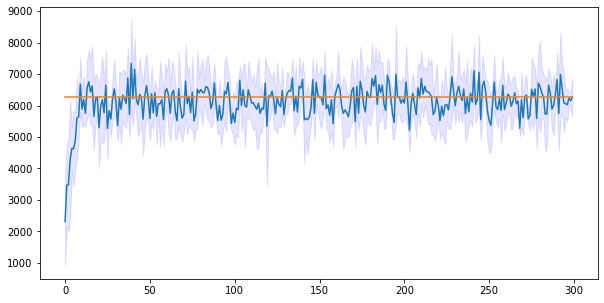
\includegraphics[width=0.6\textwidth]{img/ts_reward5.png}
    \caption{TS Reward}
    \label{fig:reward52}
    \end{center}
\end{figure}
\begin{multicols}{2}
    \begin{figure}[H]
        \begin{center}
        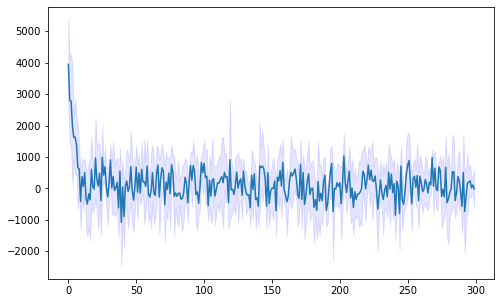
\includegraphics[width=0.5\textwidth]{img/ts_regret5.png}
        \caption{TS Regret}
        \label{fig:regret52}
        \end{center}
    \end{figure}
    \columnbreak
    \begin{figure}[H]
        \begin{center}
        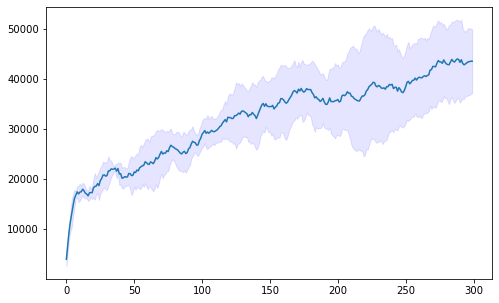
\includegraphics[width=0.5\textwidth]{img/ts_cum_regret5.png}
        \caption{TS Cumulative regret}
        \label{fig:cum_reg52}
        \end{center}
    \end{figure}
\end{multicols}